\documentclass[letterpaper,12pt]{article}
\usepackage{graphicx} % Required for inserting images
\usepackage{caption}

\title{PVZGOD}
\author{Carlos Santiago Mortera Cota}
\date{\today}

\begin{document}

\maketitle

\section{¿Por qué plantas contra zombies 1 es el mejor de todos?}
Plantas contra zombies clasico fue el mejor todos los juegos que salieron, pero, ¿por qué? bueno, esto se debe a varias razones:
\begin{itemize}
    \item El diseñador original del juego ,\textit{George Fan}, tenia propositos personales en el proyecto, por lo que era una obra con amor.
    
    \item El juego en su simplicidad ofrece bastante contenido diverzo y entretenido de forma sencilla, que es facil de entender para cualquier tipo de juagdor, sin explicaciones inecesariamente complicadas
\end{itemize}

Estos dos aspectos podran parecer de poca relevancia, pues uno pensaría que en todo proyecto tan grande como lo es un videojuego las persona detras dejan una parte de si en el, es una obra con jenuino amor por lo que se hace, esta debería ser la realidad detras de toda clase de proyectos, pero como muchas cosas en la vida, la realidad es más amarga y fea. Tristemente, como en varios casos de otros videojuegos, la distribuidora, o veces la misma desarrolladora, toman gran influencia sobre la dirección del proyecto y la visión sobre el, dajando a un lado a la gente que originalmente tenia la idea y el enfoque que hacian al videojuego bueno, esto fue lo mismo que le paso a PvZ.
\newline
¿Quien fue el verdugo de PvZ?, bueno, el \textbf{culpable fué EA} quien despues de haberse convertido en la distribuidora de PvZ, cambio completamente el enfoque de lo que siguio de la franquicia, aunque no todo fue necesariamente malo, como el cambio de arte en el PvZ 2, o la creación de los Warden Warfare, es exageradamente evidente que la intención con los siguientes juegos, con unica exepción los Warden Warfare, era sacarle la mayor cantidad de dinero al jugador, la estrategia, el free to play con servicio, donde en ves de darle prioridad a hacer un buen juego, que te motive a gastar dinero en el, hicierón algo similar a lo que hizo Rovio con angry birds 2, y se enfocaron en meter una absurda cantidad de anuncios y microtransacciones para poder desbloquerar plantas con diseños mediocres y con poco esfuerzo detras, una de las mayores proebas de esto es el PvZ 2, que a persar de tener muchas cosas rescatables, esta lleno de microtransacciones para desbloquear las plantas o subirlas de nivel para poder hacer los retos de tiempo limitado. Quedo muy marcado que ya no hacian PvZ con otro proposito que no fuera \textbf{sacarte el dinero}. Por eso la gente en su mayoria prefiere la obra original de PvZ.

\section{¿Qué mantiene vivo el gusto por pvz?}

Como muchos otros juegos, lo que a echo que de vez en cuando se escuche de PvZ fue su comunidad con la creación de mods, que son la mayoria chinos. Un ejemplo de los buenos mods que han salido es el sonado PvZ fusión, que partiendo del juego originala con sus plantas clasicas, el mod agrega la posibilidad de fusionarlas para crear nuevas plantas con poderes combinados, además de agregar unas cuantas plantas totalmemte nuevas y originales. 
\newline
\begin{figure}[h!]
\centering
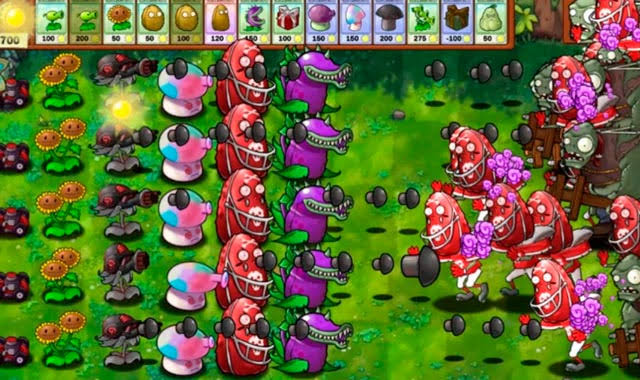
\includegraphics[scale=0.5]{PvZFusion.jpeg}
\caption{\textit{Imagen gameplay del PvZ Fusion}}
\end{figure}  
\newline
La creación de mods permite que el juego consiga nuevo contenido y por los diferentes enfoques de los creadores y sus ideas personales, hay contenido nuevo para toda clase de jugadores, y como la mayoria de los mods son chinos, hay toda clase de retos semi-imposibles de superar que son muy divertidos de intentar (almenos en mi caso), esta es la razón de que PvZ siga presente, afortunadamente es su gran comunidad la que lo mantiene relevante y activo, pues la desarrolladora Pop Cap, y la distribuidora EA no han echo nada bueno con los utimos proyectos. 


\end{document}
